\documentclass{article}

\usepackage{geometry}
\geometry{margin=2cm}
\usepackage{graphicx}
\usepackage{hyperref}

\hypersetup{colorlinks=true, linkcolor=blue, urlcolor=blue}
\urlstyle{same}
\begin{document}
	
	\author{Aayush Arya}
	\date{August 28, 2021}
	\title{}
	
	\maketitle
	
	\hrule
	\begin{center}
		PHY366 Lab Report\\
		Registration No.: 11912610 \quad Section: G2903
	\end{center}
	\hrule

	\section*{Aim}
	To design and analyse a series LCR circuit.
	
	\section*{Methods}
	
	We simulated a series LCR circuit on the online platform \textsc{MultiSim}\footnote{Constructed circuit is available at \url{https://www.multisim.com/content/XudVnEW8m4cFpayszBtMSX/lcr-series-prac-1/open/}}, employing a $20\Omega$ resistor, a 200 $\mu$H inductor and a $2.0\mu$F capacitor.
	
	\begin{figure}[h]
		\centering
		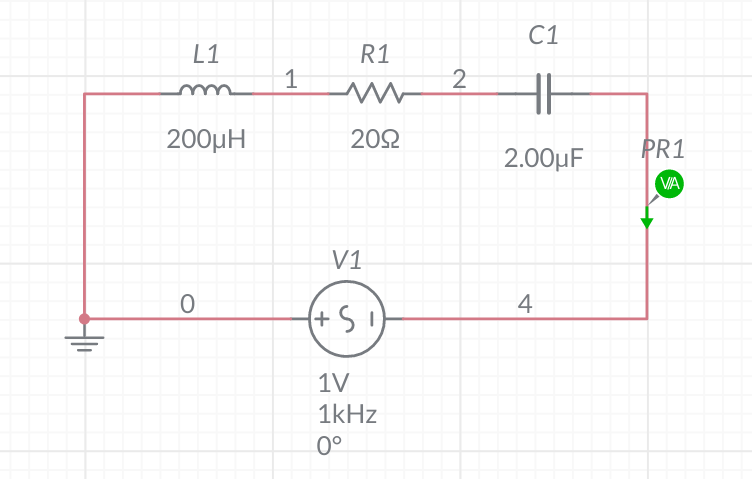
\includegraphics[width=0.6\textwidth]{../circuit}
		\label{fig:circuit}
		\caption{The series LCR circuit employed here.}
	\end{figure}

	We predict resonance at
	$$ \omega = \frac{1}{\sqrt{LC}} = \frac{1}{200\times2\times10^{-6}\times 10^{-6}} $$
	which is $\omega = 50,000$ or $f_0 = 7.96$ kHz.\\
	
	We applied a 1V AC supply and expected to get a $i_0 = 1/20 = 50$mA peak current at resonance. The circuit we used is shown in Figure 1.
	
	From the data obtained from the simulator, we also calculated the bandwidth and the corresponding quality factor of the LCR circuit. We summarize our results in the succeeding section.

	\section*{Results}
	
	We obtain a resonance peak at a frequency of $\sim 7.94$ kHz and a peak current of $50$mA, consistent with theoretical estimates (see Figure 2). A summary of the data produced by the simulator is available in the \texttt{LCR series data.csv} file included with this report.\\
	
	
	\begin{figure}[h!]
		\centering
		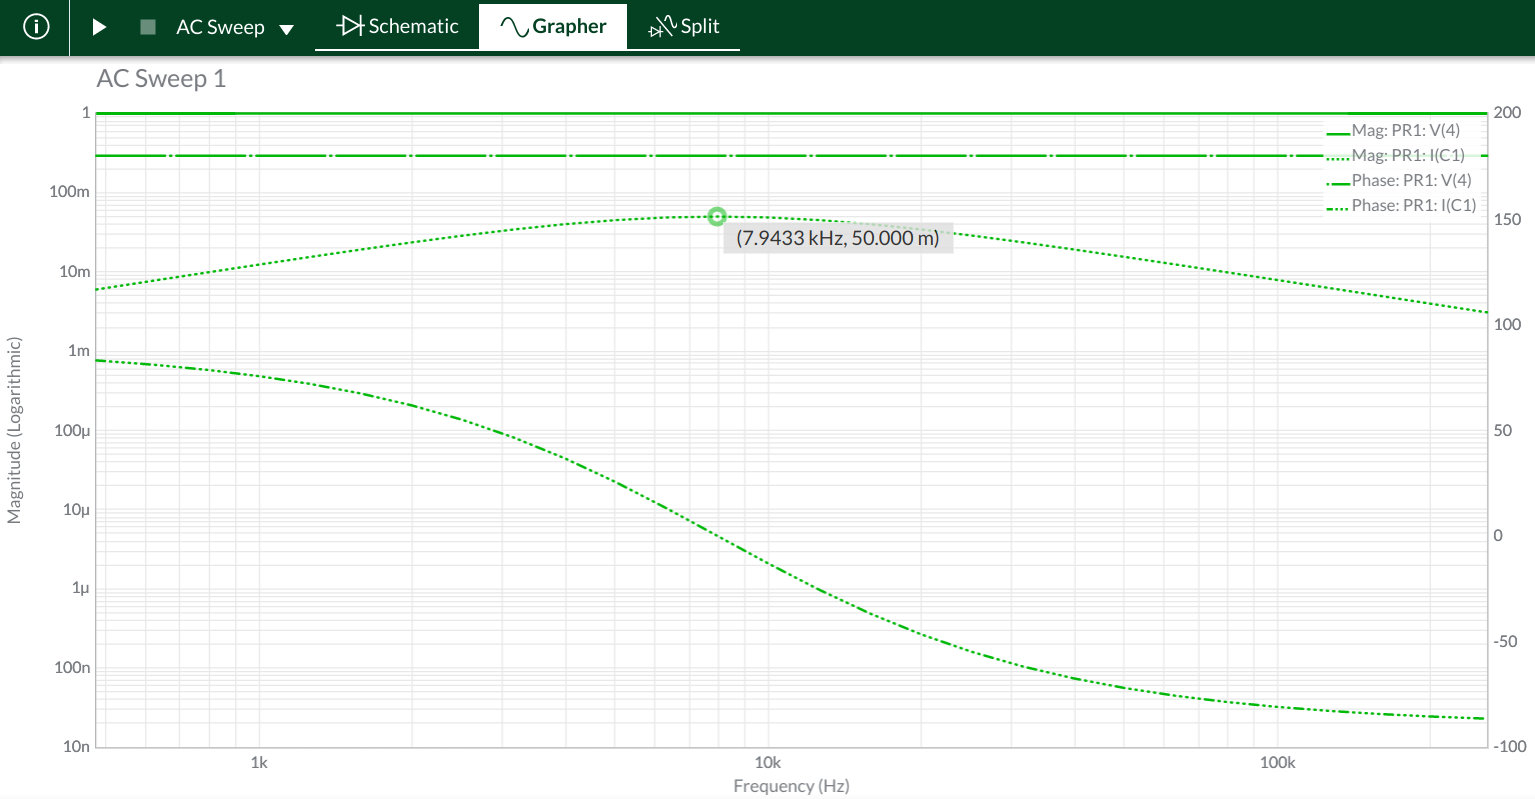
\includegraphics[width=0.7\textwidth]{../resonance_current}
		\label{fig:peak}
		\caption{The resonance peak is obtained at $\sim 7.94$kHz, consistent with the theoretical expectations.}
	\end{figure}

	The current drops to around $0.707 i_0$ at $f_1 = 3.16$ kHz and $f_2 = 19.95$ kHz respectively. From this we calculate the bandwidth to be
	$$ \mathrm{BW} = \Delta f = 19.95-3.16$$
	or $\mathrm{BW} = 16.79$ kHz.\\
	
	The quality factor $Q$ of the circuit is defined as $$ Q = \frac{f_0}{\mathrm{BW}}$$
	where $f_0$ is the resonance frequency (here, $7.94$kHz).
	
	This gives a Q-value of $Q \sim 0.47$.
	
\end{document}
